\documentclass[tikz]{standalone}
\usepackage{pgfplots}
\usepgfplotslibrary{groupplots}
\pgfplotsset{width=8.4cm, height=7cm, compat=1.18}
\usepackage{tikz}
\usepackage{circledsteps}
\usepackage{gensymb}
\usepackage{amsmath}
\usetikzlibrary{calc}
\usepackage[outline]{contour}
\contournumber{64}% default is 16, star form uses 32
\contourlength{.12em}% default is 0.03em
\usetikzlibrary {arrows.meta} 
\usetikzlibrary{decorations.pathreplacing, calligraphy}

\thinmuskip=2mu
\medmuskip=2mu
\thickmuskip=2mu
\def\phival{45}
\def\thetaval{-45}
\def\radiusval{1.5}
\def\outradiusval{2.}
\def\textmargin{0.4}
\def\anglemargin{5}
\def\centerarc[#1](#2)(#3:#4:#5)% Syntax: [draw options] (center) (initial angle:final angle:radius)
{ \draw[#1] ($(#2)+({#5*cos(#3)},{#5*sin(#3)})$) arc (#3:#4:#5); }

\def\myline{very thick}

\begin{document}
% This file was created with tikzplotlib v0.10.1.
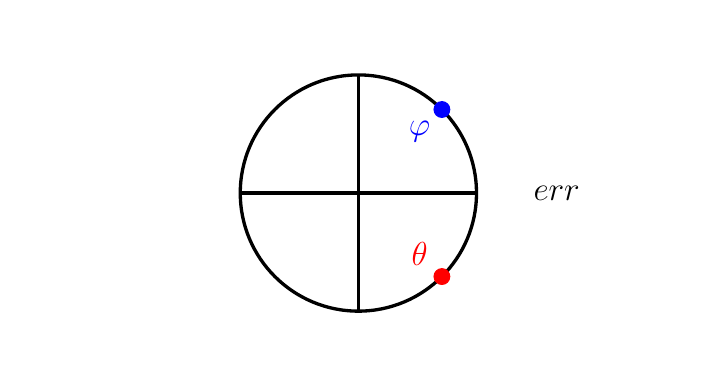
\begin{tikzpicture}
	\useasboundingbox (-4.2,-\outradiusval-0.1) rectangle (4.2,\outradiusval+0.1);
	\definecolor{darkgray176}{RGB}{176,176,176}
	\definecolor{darkred}{RGB}{139,0,0}
	\definecolor{lightgray204}{RGB}{204,204,204}
	\definecolor{darkgray140}{RGB}{140,140,140}
	\definecolor{lightred}{RGB}{255,150,150}
	\definecolor{darkgreen}{RGB}{0,150,0}
	% Canvas
	\draw[\myline] (-\radiusval,0) -- (\radiusval,0);
	\draw[\myline] (0,-\radiusval) -- (0,\radiusval);
	\draw[black,\myline] (0,0) circle (\radiusval cm);
	% Points and texts
	\draw[fill=red, draw=red, anchor=center] ({\radiusval*cos(\thetaval)},{\radiusval*sin(\thetaval)}) circle (0.1cm);
	\draw[fill=blue, draw=blue, anchor=center] ({\radiusval*cos(\phival)},{\radiusval*sin(\phival)}) circle (0.1cm);
	\node[red, anchor=center] at ({(\radiusval-\textmargin)*cos(\thetaval)},{(\radiusval-\textmargin)*sin(\thetaval)}) {\large{$\theta$}};
	\node[blue, anchor=center] at ({(\radiusval-\textmargin)*cos(\phival)},{(\radiusval-\textmargin)*sin(\phival)}) {\large{$\varphi$}};
	\node[anchor=west] at ({(\outradiusval+0.1)*cos(\phival + \thetaval)},{(\outradiusval+0.1)*sin(\phival + \thetaval)}) {\large{$err$}};
	% Arrowed art
	\centerarc[\myline, stealth-stealth](0,0)({\thetaval+\anglemargin}:{\phival - \anglemargin}:\outradiusval cm)
	\centerarc[\myline, dashed, stealth-stealth](0,0)({\phival + \anglemargin}:{360+\thetaval-\anglemargin}:\outradiusval cm)
	
\end{tikzpicture}


\end{document}